\begin{frame}{第十三讲、导数与微分}
	\linespread{1.5}
	\begin{enumerate}
	  \item {\bf 内容与要求}{\b( \S4.2-4.3 )}
	  \begin{itemize}
	    \item 掌握隐函数和参数方程的求导方法
% 	    \begin{itemize}
% 	      \item 了解隐函数和参数方程的高阶导数计算方法
% 	    \end{itemize}
	    \item 理解微分的概念
	    \item 掌握微分法则
% 	  \vspace{1em}
	  \end{itemize}
	  \item {\bf 课后练习:}
	  \begin{itemize}
	    \item 书面作业:{\b 习题4.2:10,11,14,15;习题4.3:3,4,8,11}
	    \item 思考题:{\b 习题4.2:16,17,19;习题4.3:2,9,10,12-14}
	  \end{itemize}
	\end{enumerate}
\end{frame}

\section{隐函数求导法则}

\begin{frame}{隐函数求导法则}\pause 
	\linespread{1.2}
	{\bf 隐函数:}由形如$f(x,y)=0$的方程所确定的函数\pause 
	\begin{columns}
		\column{.5\textwidth}
			\begin{exampleblock}{{\bf 例1}\hfill P185-例28}
				设$y=y(x)$是由方程
				$$x^3+y^3=3xy$$
				所确定的隐函数,满足$y(3/2)=3/2$,求其
				在点$(3/2,3/2)$处的切线方程。
			\end{exampleblock}\pause 
		\column{.45\textwidth}
			\begin{center}
				\resizebox{!}{5cm}{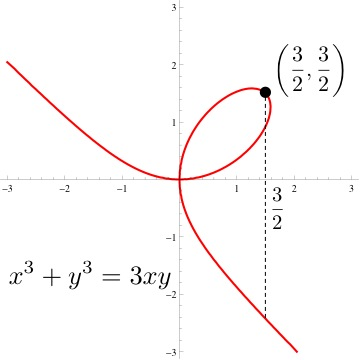
\includegraphics{./images/ch4/x3y33xy.jpg}}
			\end{center}
	\end{columns}
\end{frame}

\begin{frame}
	\linespread{1.5}
	\begin{exampleblock}{{\bf 例2}\hfill P186-例29}
		设$y=y(x)$是由方程$y^2=x^2-\cos y$所确定的隐函数,求$y''(x)$。
	\end{exampleblock}\pause 
	\begin{center}
		\resizebox{!}{6cm}{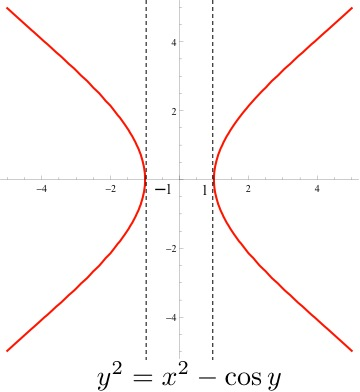
\includegraphics{./images/ch4/y2x2-cosy.jpg}}
	\end{center}
\end{frame}

\begin{frame}{利用隐函数求导法简化求导运算}
	\linespread{1.2}\pause 
	\begin{exampleblock}{{\bf 例3}\hfill P187-例30}
		求函数$y=(x^2+1)\sqrt[3]{(x-2)^2(x^2+x)}$的导数。
	\end{exampleblock}
\end{frame}

\section{参数方程求导法则}

\begin{frame}{参数方程求导法则}
	\linespread{1.2}\pause 
	设函数$y=y(x)$由参数方程
	$$\left\{
	\begin{array}{l}
	x=\varphi(t)\\
	y=\psi(t)
	\end{array}
	\right.$$
	确定,\pause $x=\varphi(t)$可逆,\pause 则
	$$y'(x)=\df{\psi'(t)}{\varphi'(t)}$$\pause 
	\begin{exampleblock}{{\bf 例4}\hfill P188-例31}
		求抛物线$x=y^2$在$(1,1)$和$(4,-2)$处的切线方程。
	\end{exampleblock}
\end{frame}

\begin{frame}
	\linespread{1.2}
	\begin{exampleblock}{{\bf 例5}\hfill P189-例32}
		已知$\left\{
	\begin{array}{l}
	x=t-\sin t\\
	y=1-\cos t
	\end{array}
	\right.$,求$y''(x)$。
	\end{exampleblock}\pause 
	\begin{center}
		\resizebox{!}{4cm}{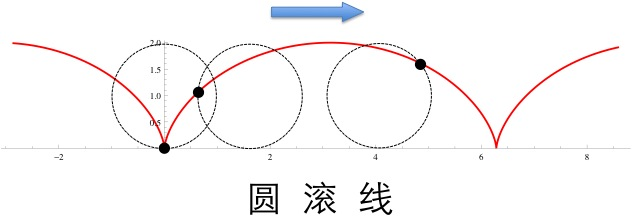
\includegraphics{./images/ch4/sphereRoll.jpg}}
	\end{center}
\end{frame}

\section{微分的概念}

\begin{frame}{“以直代曲”与局部线性化}
	\linespread{1.2}\pause 
	若$f(x)$在$x_0$可导,则
	$$f(x)=f(x_0)+f\,'(x_0)(x-x_0)+\circ(x-x_0)\quad(x\to x_0)$$\pause 
	即:\alert{在$x_0$附近,$f(x)$可以近似地表示为一个线性函数}\pause 
	$$f(x)\approx f(x_0)+f\,'(x_0)(x-x_0)$$\pause 
	\vspace{-2em}
	\begin{exampleblock}{{\bf 例6}\hfill P200-例5}
		在截面半径$r=0.12cm$,长$l=4cm$的圆柱体侧面镀铜(比重$\rho=8.9g/cm^3$),
		若镀层厚度$\Delta r=0.001cm$,约需要多少克铜(近似到小数点后4位)?
	\end{exampleblock}
\end{frame}

\begin{frame}{微分的概念}
	\linespread{1.2}\pause 
	\begin{block}{{\bf 定义4.3.1}\hfill P195}
		设$y=f(x)$在$x_0$的某领域内有定义,若存在与$\Delta x$无关的常数$A$,使得$\Delta y=f(x_0+\Delta
		x)-f(x_0)$满足
		 $$\Delta y=A\Delta x+\circ(\Delta x)\;(\Delta x\to 0)$$\pause 
		则称$y=f(x)$在$x_0${\bb 可微},\pause $A\Delta x$称为{\bb $y=f(x)$在$x_0$处的微分},\pause
		记为 $$\left.\d y\right|_{x=x_0}\quad \mbox{或} \quad
		\left.\d f(x)\right|_{x=x_0}$$
	\end{block}
\end{frame}

\begin{frame}{可微与可导的关系}
	\linespread{1.2}\pause 
	\begin{block}{{\bf 定理4.3.1}\hfill P195}
		设$y=f(x)$在$x_0$可微,当且仅当$y=f(x)$在$x_0$可导,且
		$$\left.\d y\right|_{x=x_0}=f\,'(x_0)\d x\quad 
		\mbox{或} \quad
		\left.\d f(x)\right|_{x=x_0}=f\,'(x_0)\d x$$
	\end{block}\pause 
	\begin{exampleblock}{{\bf 例7}\hfill P196-例3}
		设$f(x)=x^3+2x^2-3x+6$,求$\d f(x)$和$\d f(x)|_{x=1}$,并求其在$(1,6)$
		处的局部线性化函数$L(x)$。
	\end{exampleblock}
\end{frame}

\begin{frame}{微分运算法则}
	\linespread{1.2}\pause 
	\begin{block}{{\bf 定理4.3.2}(四则运算)\hfill P200}
		设$u(x),v(x)$可导,则
		\begin{enumerate}
		  \item $\d (u\pm v)=\d u\pm \d v$
		  \item $\d(uv)=v\d u+u\d v$
		  \item $\d\df uv=\df{v\d u-u\d v}{v^2}$
		\end{enumerate}
	\end{block}\pause 
	\begin{block}{{\bf 定理4.3.3}(复合运算)\hfill P201}
		设$y=f(u),u=\varphi(x)$均可微,则$y=f[\varphi(x)]$可微,
		$$\d y=f\,'(u)\d u=f\,'(u)\varphi'(x)\d x$$
	\end{block}
\end{frame}

\begin{frame}
	\linespread{1.2}
	\begin{exampleblock}{{\bf 例8}\hfill P201-例6}
		求函数$y=e^{2x-1}\sin x$的微分。
	\end{exampleblock}\pause 
	\begin{exampleblock}{{\bf 例9}\hfill P202-例7}
		试将下列微分形式表示为某一函数的微分\pause 
		\begin{enumerate}
		  \item $x^2\d x$\pause 
		  \item $e^{2x}\d x$\pause 
		  \item $\cos(5x-1)\d x$\pause 
		  \item $\df{1}{1+2x^2}\d x$
		\end{enumerate}
	\end{exampleblock}
\end{frame}

\begin{frame}[<+->]{小结}
	\linespread{2}
	\begin{enumerate}
	  \item {\bf 隐函数和参数方程的求导方法}
	  \begin{itemize}
	    \item 高阶导数的计算方法
% 	    \item 反函数
% 	    \item 复合函数
	  \end{itemize}
	  \item {\bf 微分的概念}
	  \begin{itemize}
	    \item 可微与可导的关系
	    \item 微分的不变性
	  \end{itemize}
% 	  \item {\bf 高阶导数}
% 	  \begin{itemize}
% 	    \item 一些特殊函数的高阶导数
% 	  \end{itemize}
	\end{enumerate}
\end{frame}

\begin{frame}{问题讨论}
	\linespread{1.5}
	\begin{enumerate}\pause 
	  \item 若$f(x),g(x)$在$x_0$均不可导,是否$f(x)+g(x),$ $f(x)g(x)$必不可导?\pause
	  (\alert{$\times$})\pause 
	  \item 若对任意$x\in (a,b)$,恒有$f(x)<g(x)$,且$f(x),g(x)$均在$(a,b)$内
	  可导,问是否必有$f\,'(x)<g'(x)$?\pause (\alert{$\times$})\pause 
	  \item 若$f(x)$在$\mathbb{R}$上可导,且$\limx{+\infty}f(x)=\infty$,是否
	  必有$\limx{+\infty}f\,'(x)=\infty$?\pause (\alert{$\times$})
	\end{enumerate}
\end{frame}

\begin{frame}{问题讨论}
	\linespread{1.5}\pause 
	\begin{enumerate}
	  \addtocounter{enumi}{3}
	  \item 若$f(x)$在$(a,b)$内可导,且$\limx{a^+}f(x)=\infty$,是否
	  必有$\limx{a^+}f\,'(x)=\infty$?\pause (\alert{$\times$})\pause 
	  \item 若$f(x)$可导且为奇(偶)函数,则$f\,'(x)$也有奇偶性?\pause (\alert{$\surd$})\pause 
	  \item 若$f(x)$可导且为周期函数,则$f\,'(x)$也是周期函数?\pause (\alert{$\surd$})
	\end{enumerate}
\end{frame}

\begin{frame}
	\linespread{1.2}
	\begin{exampleblock}{{\bf 例1}\hfill P211-习题7}
	下图包含了沿坐标轴轴线运动物体的位置$s(t)$,速度$v(t)$和加速度$a(t)$的函数图形,试
	根据图形特征指出每条曲线对应的函数分别是什么。
	\begin{center}
		\resizebox{!}{5cm}{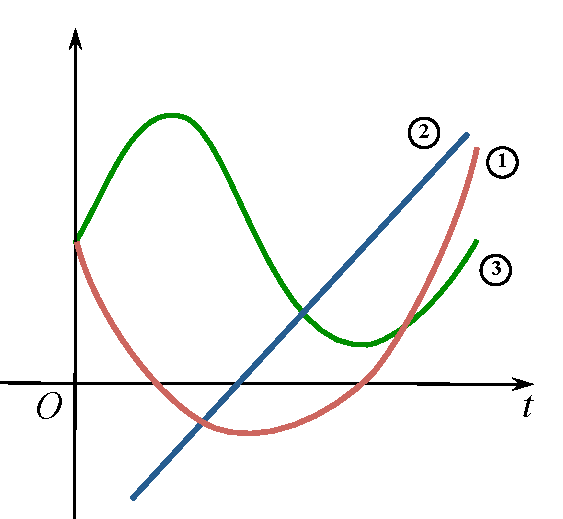
\includegraphics{./images/ch4/ffa.pdf}}
	\end{center}
	\end{exampleblock}
\end{frame}

% \section{补充例题}

% \begin{frame}{补充例题}
% 	\linespread{1.5}
% 	\begin{exampleblock}{{\bf 例2}\hfill }
% 		设$f(x)=|x+1|^3-2$,试求$f\,'(x),f\,''(x)$,又问$f\,'(-1),f\,''(-1),f\,'''(-1)$
% 		是否存在?
% 	\end{exampleblock}\pause 
% 	\begin{exampleblock}{{\bf 例3}\hfill }
% 		计算$f\,'(x)$,已知
% 		$$f(x)=\left\{\begin{array}{ll}
% 		x^2e^{-x^2},& |x|\leq 1\\
% 		1/e,& |x|>1
% 		\end{array}
% 		\right.$$
% 	\end{exampleblock}
% \end{frame}

\begin{frame}
	\linespread{1.5}
	\begin{exampleblock}{{\bf 例2}\hfill }
		设$f(x)=\left\{\begin{array}{ll}
		\df{1-\sqrt{1-x}}{x}, & x<0,\\
		a+bx, & x\geq 0
		\end{array}\right.$,求$a,b$使$f(x)$处处可导。
	\end{exampleblock}\pause 
	\begin{exampleblock}{{\bf 例3}\hfill }
		设$\left\{\begin{array}{l}
		x=f\,'(t)\\ y=tf\,'(t)-f(t)
		\end{array}\right.$,求$\df{\d^2y}{\d x^2}$,其中$f\,''(x)$存在且不为零。
	\end{exampleblock}
\end{frame}

\begin{frame}
	\linespread{1.5}\pause 
	\begin{exampleblock}{{\bf 例4}\hfill }
		证明过曲线$\sqrt x+\sqrt y=\sqrt a$上任一点$(x_0,y_0)$的切线在两坐标轴上
		的截距之和为常数。
	\end{exampleblock}\pause 
	\bigskip
	\begin{exampleblock}{{\bf 例5}\hfill }
		求函数$y=\df{1}{x^2-3x-4}$的$n$阶导函数。
	\end{exampleblock}\pause 
\end{frame}

\begin{frame}
	\linespread{1.5}\pause 
	\begin{exampleblock}{{\bf 例6}\hfill }
		设$y=\arctan x$,求$y^{(n)}(0)$
	\end{exampleblock}\pause 
	\bigskip
	\begin{exampleblock}{{\bf 课后思考题}\hfill 习题集P77-例23}
		设$y=(\arcsin x)^2$,求$y^{(n)}(0)$
	\end{exampleblock}
\end{frame}

%====================================

% \begin{frame}{title}
% 	\linespread{1.2}
% 	\begin{block}{{\bf title}\hfill}
% 		123
% 	\end{block}
% \end{frame}